\documentclass[12pt]{article}
\usepackage{amsmath,amsthm,amssymb}
\usepackage{booktabs}
\usepackage{hyperref}
\usepackage{graphicx}
\usepackage{float}

\begin{document}
\title{AI Homework 6}
\author{Jinhui Zhang\\
jinhzhan@indiana.edu}  
\maketitle
\begin{enumerate}
\item \textbf{What is your criterion for ``sufficiently similar", and what considerations led you to choose it?}\\
My answer: My criterion is the Manhattan distance between two states. According to heuristic functions used in 8-puzzle problem, Manhattan distance can measure the difference between two states more accurately. Though there is a better strategy, that is, separate one state into two parts in which there is a four numbers and calculate the Manhattan distance, it would take a long time for the separation and calculation. For the consideration of time, Manhattan distance is, I think, a nice tradeoff between speed and accuracy. 

\item \textbf{What is your criterion for quality of solutions generated?  }\\
My answer: I use the time cost and the number of states generated to measure the quality of solutions. Both of time and space are taken into account. 

\item \textbf{Briefly describe your experimental design.}\\
My answer: I use the initial states from 1 to 15 in \href{http://www.cs.indiana.edu/classes/b551/sample8puzzleStates.py}{this link} to generate case base. Then I design four sets of test cases: dissimilar and hard, similar and easy, dissimilar and easy, and similar and hard. There are five cases in each set. The goal states are all the same: (1, 2, 3, 4, 5, 6, 7, 8, "blank"). And run case based reasoning and informed search code separately. Here the informed search only use Manhattan distance. Then compare the time cost and number of runs. For those cases are not similar with these in the casebase, I directly use scratch to find the solution path. 

\item \textbf{Generate and include graphs for each of the 4 states in \{easy, hard\} x \{similar input problems, dissimilar input problems\}.}\\
My answer: In my experiment, the test cases from 1 to 5 is dissimilar and hard, from 6 to 10 is similar and easy, from 11 to 15 is dissimilar and easy, from 16 to 20 is similar and hard. 
\begin{figure}[H]
\centering
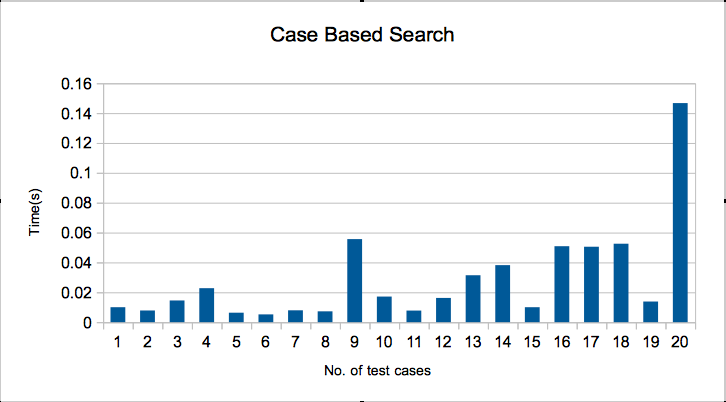
\includegraphics[width=0.8\textwidth]{Time_case.png}
\caption{Time cost in case based reasoning}
\label{fig:Time_case}
\end{figure}
\begin{figure}[H]
\centering
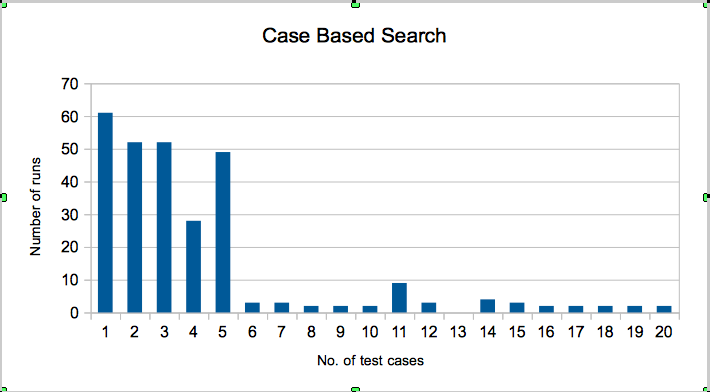
\includegraphics[width=0.8\textwidth]{Number_case.png}
\caption{Numbers of runs in case based reasoning}
\label{fig:Num_case}
\end{figure}
Notice that although in figure\ref{fig:Time_case}, the time cost is a little longer than that in informed search, in figure\ref{fig:Num_case} the number of runs is much less. Because I use a file named "casebase" to store all old cases, the time is mainly occupied by I/O operation. In figure\ref{fig:Num_case} we can see that in case 1 to 5, they are all dissimilar and hard, so my program calls informed search, and the number of runs is distinctly greater than the others. For case 11 to 15, they are also dissimilar, but these cases are easy ones. So the number of runs is a little higher(just ignore case 13). Hence, in the view of combination of time and space cost, case based reasoning is acceptable for looking for a solution. 
\begin{figure}[H]
\centering
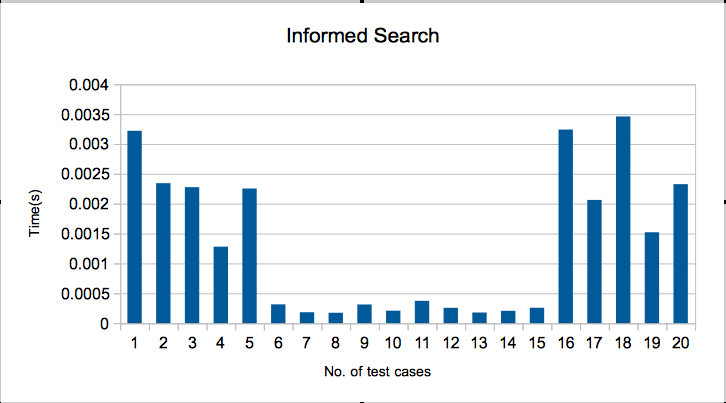
\includegraphics[width=0.8\textwidth]{Time_informed.png}
\caption{Time cost in informed search}
\label{fig:Time_info}
\end{figure}
\begin{figure}[H]
\centering
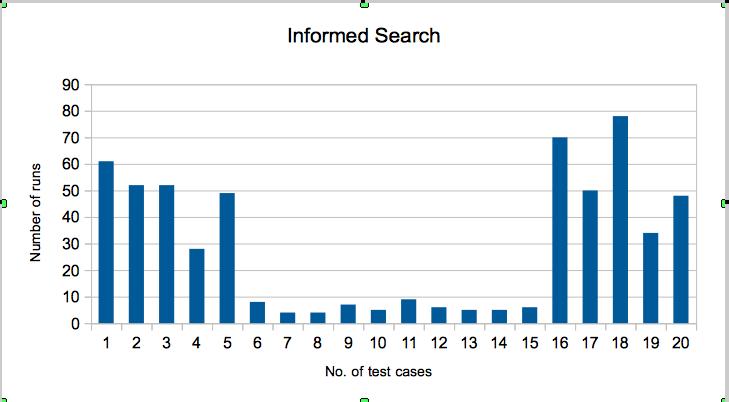
\includegraphics[width=0.8\textwidth]{Number_informed.png}
\caption{Numbers of runs in informed search}
\label{fig:Num_info}
\end{figure}
Then as to informed search, in figure\ref{fig:Time_info}, time cost is better than that in case based reasoning. The reason is that informed search doesn't have I/O operation. So it doesn't need that much time. However, when it comes to the number of runs, informed search needs more generated states cause it doesn't have a storage mechanism to keep old cases in mind. 

\item \textbf{Describe what your experimental results show about the tradeoffs of using CBR:}
\begin{enumerate}
\item When is performance in the learning system better than the hw3 system, and when is it worse?\\
My answer: When it is similar and hard, the performance in learning system is much better than the hw3 system. And when it is similar and easy, the advantage of learning system is not that clear. When it is dissimilar and no matter if it is easy or hard, the performance in the learning system is worse than the hw3 system. That is because when it is dissimilar, before the learning system calls informed search, it tries to find a similar case in case base. The I/O operation need time to execute. 
\item What are the time/space overhead issues from your system?s learning?\\
My answer: We can check the cases from 1 to 5 and from 11 to 15. They are all dissimilar. So the time for learning system is overhead + informed search. Do subtraction and average the result, time overhead is about 0.04 seconds. That means the I/O operation in learning system needs extra 0.04 seconds. 
\item How might the drawbacks be addressed? \\
My answer: In my opinion, the I/O operation cannot be avoided in learning system. Because if we need a larger data set, the embedded code that generates data is not efficient to handle this set. But we can use a database to store those data. Database is created for data operation. Its performance is much better than a plain text file. In coding level, we can consider implementing this system in a more efficient way like parallel programming. 
\end{enumerate}
\end{enumerate}
\end{document}